\chapter{Introduction}
\label{chap:introduction}

In this report, a novel method to eliminate the 6\textsuperscript{th} harmonic component on the DC link generated by the three-phase rectifier in an integrated modular motor drive (IMMD) application. Natural-commutated three-phase passive rectifiers create a harmonic component, which is 6 times the grid frequency, due to their nature of operation. Due to being a relatively low frequency component compared with the conventional switching frequencies, minimizing this harmonic component on DC link voltage and current requires bulky and costly DC link filters. In IMMD applications, decreasing the volume of passive components critical for two reasons. The first one is that, in a standard power electronics converter, passive elements constitute around 30\% of the overall volume. Secondly, the space that the integrated motor drive can be placed is small.


\begin{figure}[htp]
  \centering
  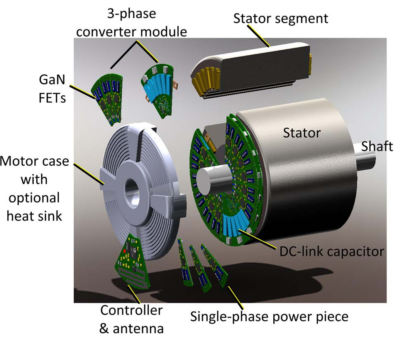
\includegraphics[width=8cm]{images/immd_concept}
  \caption{An IMMD example \cite{Wang2014}}
  \label{fig:immd_concept}
\end{figure}

An IMMD consists of a number of identical modules as shown in Fig. \ref{fig:immd_concept} \cite{Wang2014}. Each module is composed of a stator pole with concentrated coil and a drive unit and its controller dedicated to that stator pole. Having this modular structure with multiple modules brings flexibility to the designer regarding the connection of the motor drive modules on the DC link. In addition, several techniques such as interleaving can be applied for ripple and harmonic component minimization. However, all the methods developed so far are related to the switching frequency. There have been several studies in the literature for the minimization of switching frequency components on the DC link to enhance the power density of the DC link capacitors, however none of them include the effect of 6\textsuperscript{th} harmonic component due to the rectifier. In Dc link capacitor optimization studies, the effect of rectifier harmonics are neglected, and the input side is treated as an ideal DC source, which is not the case in practice.

In this research work, the modular structure is utilized with low order harmonic injection for the cancellation of the 6\textsuperscript{th} harmonic component on the DC link. First, the frequency components are modeled analytically and it is shown that a zero sequence 3\textsuperscript{th} harmonic injection by the motor drive inverters can generate a 6\textsuperscript{th} harmonic component while 2\textsuperscript{nd} and 4\textsuperscript{th} harmonic components are cancelled with a balanced three-phase inverter topology. Then, a mathematical model for the rectifier and DC link LC filter is obtained. These analytical models are verified by simulations carried out in MATLAB/Simulink. Finally, it is shown that, a significant reduction on the DC link capacitor can be achieved with this method and it is verified by simulations.

The report is organized as follows: In section 2, a description of the system is presented and the 6\textsuperscript{th} harmonic problem is shown. In section 3, the mathematical model developed for the harmonic components is presented. In section 4, the third harmonic injection method is explained to cancel the sixth harmonic component. In section 5, simulation results are presented and in section 6, general comments on the results are made.


% Burda ref ver

% Motor'a etkilerini incele (future work)
% Possible module sayıları
% Possible motor bağlantıları


